\section{Obstruction of the inherited tilted bore}\label{sec:bore}
The original upper child's inherited central axis is the line through
$t=(1,0,h)$ with unit direction $v=(\sin\alpha,0,\cos\alpha)$.
For a point $P=(x,y,z)$ define inward travel and perpendicular distance by
\[
T(P)=-v\cdot(P-t),\qquad
D(P)^2=[\cos\alpha(x-1)-\sin\alpha(z-h)]^2+y^2.
\]
For bore radius $0.0058$, the first intrusion is
$\min\{T(P):P\in K,\ D(P)\le0.0058\}$.
The certificate encloses it in $[1.325115,1.325120]$ at the reference and
in $[1.320,1.330]$ uniformly on the family. Lobes 1 and 5 intrude in the
upper bore; central inversion gives lobes 4 and 2 for the lower bore.
At the reference, the first occupied axis cross-section is near
$(0.33814,0,-0.44088)$.

An actual point with address $1404022400020420424\,0^\infty$ is inside the
reference bore, near $(0.340917,0.004592,-0.442484)$. Its mirror supplies
the other intrusion. This proves nonemptiness of the compact minimisation
set. The lower travel bound follows by discarding word balls from
\eqref{eq:tail} that lie outside the bore or beyond the proposed threshold;
all remaining reference branches close by depth 16. A separate addressed
witness supplies the uniform upper bound.

\begin{figure}[tb]
\centering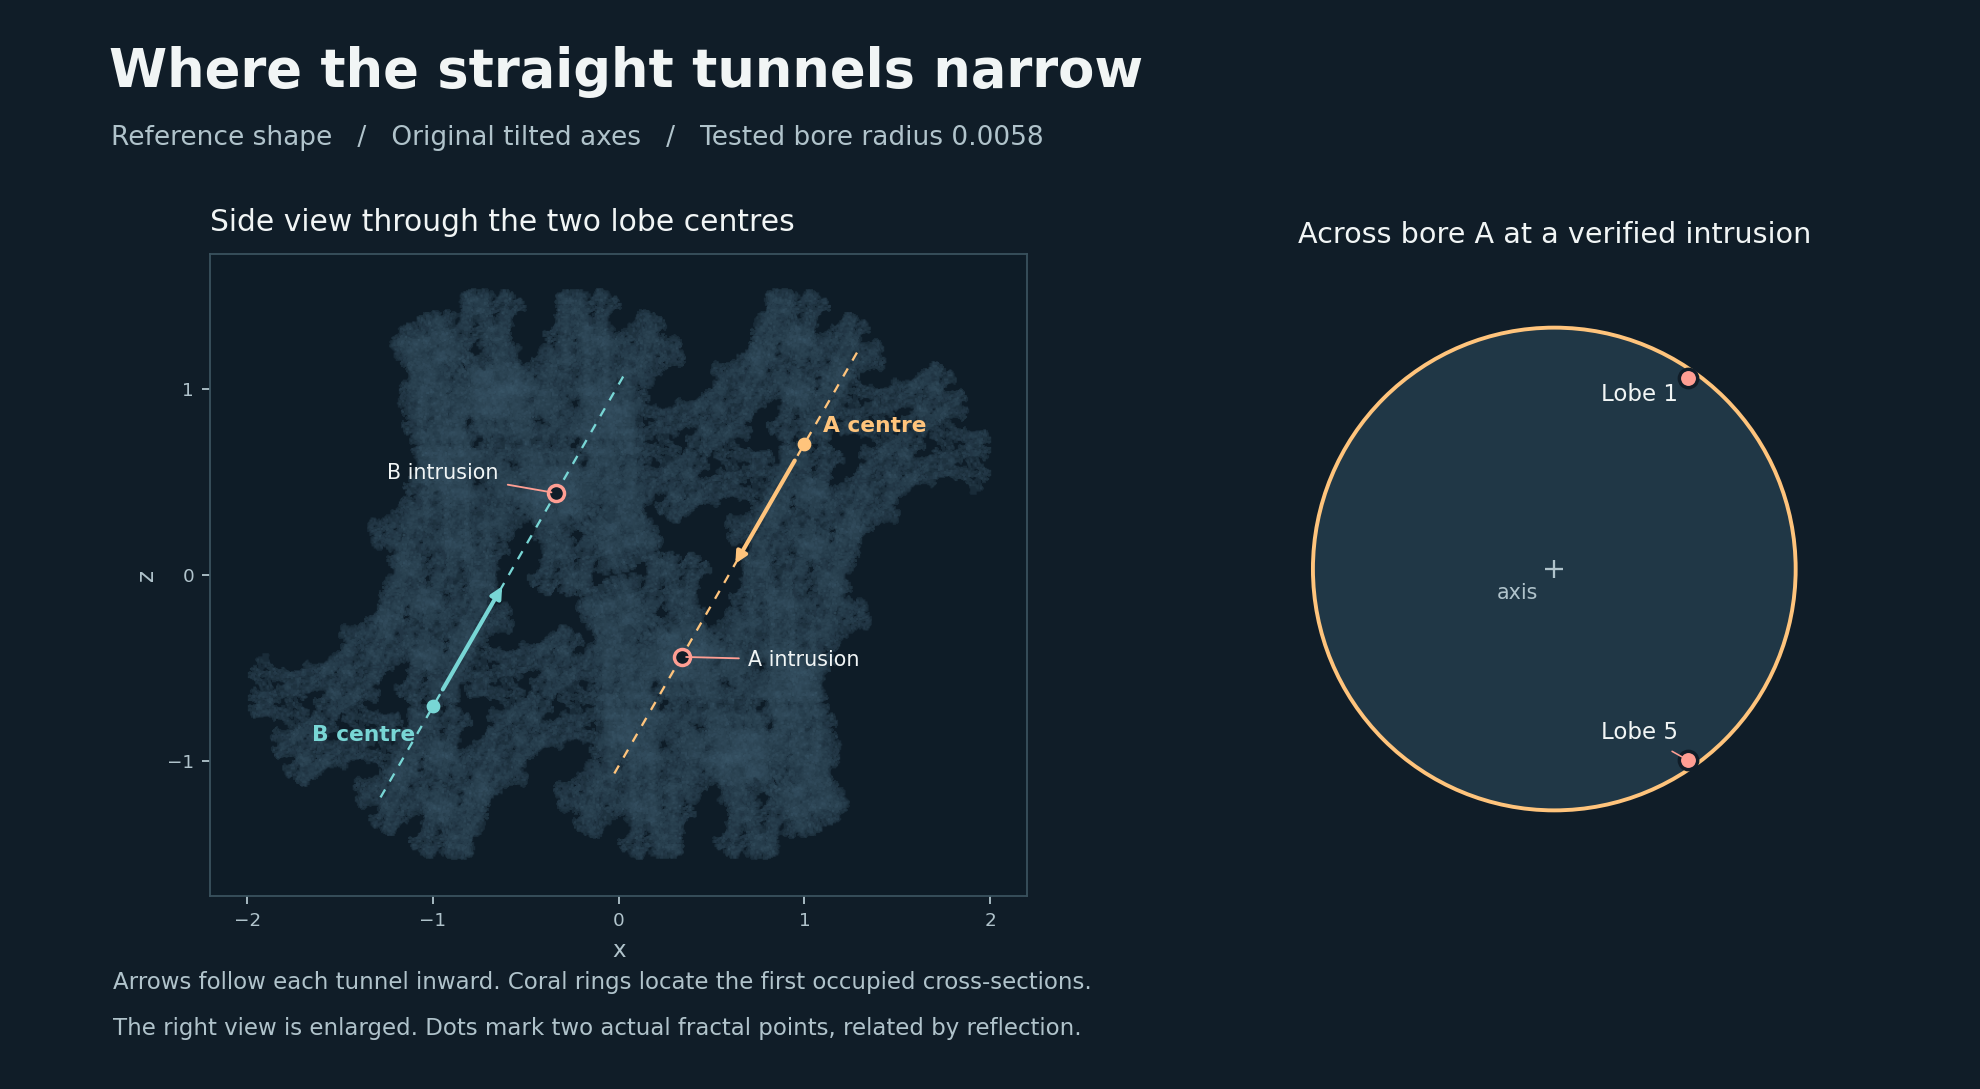
\includegraphics[width=\linewidth]{../research/fractal_research_10_topology/straight_axis_locator.png}
\caption{Obstruction of the inherited tilted bores at radius $0.0058$.
The enlarged cross-section marks actual addressed fractal points in lobes
1 and 5. Occupation of a positive-radius bore does not establish an exact
intersection with its centreline.}
\label{fig:bore}
\end{figure}

Whether the zero-width inherited axis meets $K$ remains open. Extremely close
addressed points and surviving branches of a finite search do not prove an
exact hit. The clear lines~\eqref{eq:axes} and Theorem~\ref{thm:homology} do
not depend on resolving this question. Here a ``tunnel'' denotes a certified
passage in the complement accompanied by a detected loop; it does not assume
a smooth wall or a solid body with a well-defined genus.
